\documentclass{beamer}

\usepackage{listings}
\usepackage{tikz}
\usepackage{tabularx}
\usepackage{booktabs}
\usepackage{numprint}
\usepackage{color}
\usepackage{colortbl}
\usepackage{soul}

\beamertemplatenavigationsymbolsempty

\setbeamertemplate{bibliography item}[text]
%\setbeamertemplate{bibliography entry title}{}
\setbeamertemplate{bibliography entry location}{}
\setbeamertemplate{bibliography entry note}{}

\lstset{language=Java,backgroundcolor=\color{white},keywordstyle=\color{blue}\bf,frame=single,tabsize=4}

\definecolor{light-gray}{gray}{0.9}
\newcolumntype{g}{>{\columncolor{light-gray}}r}

\makeatletter
\let\ST\st
\renewcommand\st{%
	\let\set@color\beamerorig@set@color
	\let\reset@color\beamerorig@reset@color
	\ST}
\makeatother

\setul{}{1.5pt}
\setstcolor{red}

\newcommand{\lbimpure}{Impure}

\newcommand{\lbdscsef}{Domain-spec.\,context.\,SEF}

\newcommand{\lbdsesef}{Domain-spec.\,ext.\,SEF}
\newcommand{\lbcsef}{Context.\,SEF}
\newcommand{\lbdscp}{Domain-spec.\,context.\,pure}

\newcommand{\lbdssef}{Domain-spec.\,SEF}
\newcommand{\lbesef}{Ext.\,SEF}
\newcommand{\lbdsep}{Domain-spec.\,ext.\,pure}
\newcommand{\lbcp}{Context.\,pure}

\newcommand{\lbsef}{SEF}
\newcommand{\lbdsp}{Domain-spec.\,pure}
\newcommand{\lbep}{Ext.\,pure}

\newcommand{\lbp}{Pure}

\title
{A Unified Lattice Model and \\ Framework for Purity Analyses}
\author[Helm, K\"ubler, Eichberg, Reif, Mezini] % (optional, for multiple authors)
{Dominik~Helm \and Florian~K\"ubler \and Michael~Eichberg \and Michael~Reif \and Mira~Mezini}

\date[ASE 2018] % (optional)
{
\includegraphics[scale=0.15,angle=270,origin=b]{TULogo}\raisebox{-7mm}[0pt][0pt]{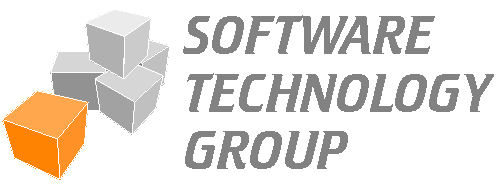
\includegraphics[scale=0.45]{logo-stg}}}

\begin{document}
	
\begin{frame}[noframenumbering]
\titlepage
\end{frame}

\setbeamertemplate{footline}{\hspace{125mm}\raisebox{2mm}[0pt][0pt]{\insertframenumber}}

\begin{frame}[fragile]
\begin{overlayarea}{\textwidth}{\textheight}
\vspace{10mm}
\begin{lstlisting}
static double radius, area;

void computeArea1(){
	area = radius * radius * Math.PI;
}

double computeArea2(){
	return radius * radius * Math.PI;
}
\end{lstlisting}
\only<2>{
\begin{itemize}
	\item Program comprehension
	\item Bug/code smell detection
	\item Optimizations
\end{itemize}
}
\end{overlayarea}
\end{frame}

\addtocounter{framenumber}{-1}

\begin{frame}[fragile]
\vspace{-2mm}
\only<1>{\vspace{21mm}}
\only<2>{
\begin{itemize}
	\item Program comprehension
	\item Optimizations
	\item Formal specification/verification
\end{itemize}
\vspace{0.35mm}
}
\begin{lstlisting}
static double radius;

double computeArea2(){
	return radius * radius * Math.PI;
}

double computeArea3(double _radius){
	return _radius * _radius * Math.PI;
}
\end{lstlisting}
\end{frame}

\begin{frame}
Unifying definitions:\\

\vspace{7mm}
\textbf{Side-effect freeness (SEF):}
\begin{itemize}
	\item execution can not be observed by other methods
\end{itemize}
\vspace{7mm}
\textbf{Purity:}
\begin{itemize}
	\item additionally deterministic
	\item i.e. can not observe the execution of other methods
\end{itemize}
\vspace{7mm}
\pause
Sufficient definitions, but valuable extensions exist
\end{frame}

\begin{frame}
\vspace{7mm}
\begin{overlayarea}{\textwidth}{0.65\textheight}
\textbf{External purity}~\cite{MostlyFunctional}:
\begin{itemize}
	\item only (observable) side-effect is modification of receiver object
	\item field setters, initialization methods, \dots
	\item respects abstraction boundaries
	\item allows finding confined side-effects
\end{itemize}
\only<2->{
\vspace{3mm}
Generalization to \textbf{contextual purity}:
\begin{itemize}
	\item side-effects restricted to parameters
	\item e.g. \texttt{System.arraycopy}
	\item allows finding more confined side-effects
\end{itemize}
}
\end{overlayarea}

\begin{thebibliography}{99999}
\bibitem[BF09]{MostlyFunctional}Benton, W.C. and Fischer, C.N. \newblock Mostly-functional behavior in Java programs, \newblock VMCAI'09
\end{thebibliography}
\end{frame}

\begin{frame}[fragile]
\textbf{Domain-specific purity:}
\begin{itemize}
	\item restricted forms of simpurity
	\item relevant for some but not all domains
	\item e.g. logging \cite{FineGrained}, exceptions
\end{itemize}
\vspace{2mm}
\begin{lstlisting}
int divide(int a, int b) {
	Log.log("Performing division");
	return a/b;
}
\end{lstlisting}
\vspace{5mm}
\begin{thebibliography}{999999}
	\bibitem[SCD16]{FineGrained}Stewart, A., Cardell-Oliver, R., Davies, R. \newblock Fine-grained classification of side-effect free methods in real-world Java code and applications to software security, \newblock ACSW'16
\end{thebibliography}
\end{frame}

\begin{frame}
\begin{overprint}
\begin{figure}[h]
	\begin{tikzpicture}[remember picture,overlay,shift={(0.2,-4)},font=\small]
	
	\node[below] (p) at (0, 6.75) {\lbp};
	
	\node[below] (sef) at (-3.5, 5.5) {\lbsef} edge[thick] (p);
	\only<4->{\node[below] (dsp) at (0, 5.5) {\lbdsp} edge[thick] (p)};
	\only<2->{\node[below] (ep) at (3.5, 5.5) {\lbep} edge[thick] (p) ;}
	
	\only<4->{\node[below] (dssef) at (-5.0, 4) {\lbdssef} edge[thick] (sef) edge[thick] (dsp)};
	\only<2->{\node[below] (esef) at (-1.63, 4) {\lbesef} edge[thick] (sef) edge[thick] (ep);}
	\only<4->{\node[below] (dsep) at (1.63, 4) {\lbdsep} edge[thick] (dsp) edge[thick] (ep)};
	\only<3->{\node[below] (cp) at (5.0, 4) {\lbcp} edge[thick] (ep);}
	
	\only<4->{\node[below] (dsesef) at (-3.5, 2.5) {\lbdsesef} edge[thick] (dssef) edge[thick] (esef) edge[thick] (dsep);}
	\only<3->{\node[below] (csef) at (0, 2.5) {\lbcsef} edge[thick] (esef) edge[thick] (cp);}
	\only<4->{\node[below] (dscp) at (3.5, 2.5) {\lbdscp} edge[thick] (dsep) edge[thick] (cp);}
	
	\only<4->{\node[below] (dscsef) at (0, 1.25) {\lbdscsef} edge[thick] (dsesef) edge[thick] (csef) edge[thick] (dscp);}
	
	\only<5->{\node[below] (impure) at (0, 0) {\lbimpure} edge[thick] (dscsef);}
	
	\end{tikzpicture}
\end{figure}
\end{overprint}
\end{frame}

\begin{frame}
\begin{overlayarea}{\textwidth}{0.8\textheight}
\vspace{4mm}
Implemented a purity analysis in OPAL\footnote[frame]{http://www.opal-project.de} that
\begin{itemize}
	\item analyses each method assuming \textbf{purity}
	\item scans the intermediate representation,\\ enriched with abstract interpretation results\\ (refined types, def-use chains, \dots)
	\item searching for counterexamples
	\item and collecting dependencies
	\item<3> which are resolved automatically
\end{itemize}
\only<2->{
\vspace{2mm}
\hspace*{-7mm}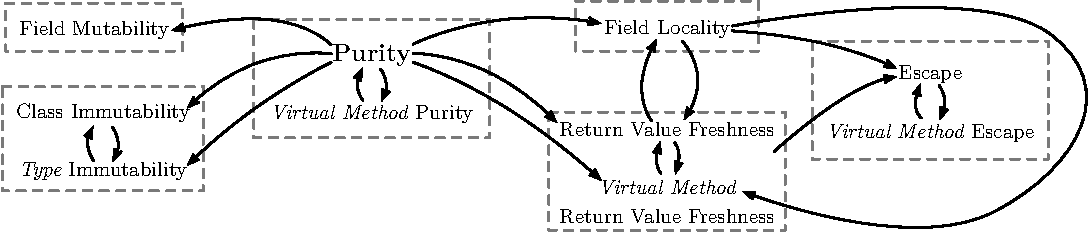
\includegraphics[scale=0.67]{AnalysisDependencies}
}
\end{overlayarea}
\end{frame}

\begin{frame}[fragile]
\vspace{2mm}
\begin{tabularx}{\textwidth}{X g>{\hspace{-7pt}}g r>{\hspace{-7pt}}r}
	\toprule
	\textbf{Corpus} & \multicolumn{2}{g}{\textbf{XCorpus}} & \multicolumn{2}{r}{\textbf{JDK8}} \\
	\emph{Methods} & \multicolumn{2}{g}{\numprint{469727}} & \multicolumn{2}{r}{\numprint{253282}} \\
	\midrule
	\lbp & \numprint{73701} & (15.69\%) & \numprint{44378} & (17.52\%) \\
	Domain-specific pure & \numprint{9628} & (2.05\%) & \numprint{8250} & (3.26\%) \\
	\midrule
	Side-Effect Free & \numprint{45268} & (9.64\%) & \numprint{18234} & (7.20\%) \\
	\lbdssef & \numprint{22056} & (4.70\%) & \numprint{14717} & (5.81\%) \\
	\midrule
	Externally pure & \numprint{19467} & (4.14\%) & \numprint{4229} & (1.67\%) \\
	Externally SEF & \numprint{2380} & (0.51\%) & \numprint{3414} & (1.35\%) \\
	\lbdsep & \numprint{639} & (0.14\%) & \numprint{354} & (0.14\%) \\
	\lbdsesef & \numprint{2467} & (0.53\%) & \numprint{1738} & (0.69\%) \\
	\midrule
	Contextually pure & \numprint{4} & (0.00\%) & \numprint{7} & (0.00\%) \\
	Contextually SEF & \numprint{7} & (0.00\%) & \numprint{48} & (0.02\%) \\
	Dom.-spec. cont. pure & \numprint{522} & (0.11\%) & \numprint{547} & (0.22\%) \\
	Dom.-spec. cont. SEF & \numprint{1523} & (0.32\%) & \numprint{1277} & (0.50\%) \\
	\midrule
	Impure & \numprint{292065} & (62.18\%) & \numprint{156089} & (61.63\%) \\
	\bottomrule
\end{tabularx}
\end{frame}

\begin{frame}[fragile]
\vspace{5mm}
\begin{tabularx}{\textwidth}{X g>{\hspace{-7pt}}g r>{\hspace{-7pt}}r}
	\toprule
	\textbf{Program} & \multicolumn{2}{>{\columncolor{light-gray}}c}{\textbf{Batik}} & \multicolumn{2}{c}{\textbf{Xalan}} \\
	\midrule
	\textbf{ReIm}~\cite{ReIm} & & & & \\
	\emph{Analyzed methods} & & \numprint{16029} & & \numprint{10386} \\
	\emph{At least Side-Effect Free} & \numprint{6072} & (37.88\%) & \numprint{3942} & (37.95\%) \\
	\arrayrulecolor{black!30}\midrule\arrayrulecolor{black}
	\emph{Execution time} & & 103s & & 140s \\
	\midrule
	\textbf{OPIUM} & & & & \\
	\emph{Analyzed methods} & & \numprint{15911} & & \numprint{10763} \\
	\emph{At least Side-Effect Free} & \numprint{6780} & (42.61\%) & \numprint{4390} & (40.79\%) \\
	\emph{Pure} & \numprint{4009} & (25.20\%) & \numprint{2492} & (23.15\%) \\
	\emph{Ext./Context. Pure/SEF} & +987 & (6.20\%) & +748 & (6.95\%) \\  \arrayrulecolor{black!30}\midrule\arrayrulecolor{black}
	\emph{Execution time} & & 197\,s & & 187\,s \\
	\bottomrule
\end{tabularx}
\vspace{5mm}
\begin{thebibliography}{999999}
\bibitem[HM12]{ReIm}Huang, W. and Milanova, A. \newblock ReImInfer: Method purity inference for Java \newblock FSE'12
\end{thebibliography}
\end{frame}

\addtocounter{framenumber}{-1}

\begin{frame}[fragile]
\vspace{5mm}
\begin{tabularx}{\textwidth}{X g>{\hspace{-7pt}}g r>{\hspace{-7pt}}r}
	\toprule
	\textbf{Program} & \multicolumn{2}{>{\columncolor{light-gray}}c}{\textbf{Batik}} & \multicolumn{2}{c}{\textbf{Xalan}} \\
	\midrule
	\textbf{ReIm}~\cite{ReIm} & & & & \\
	\emph{Analyzed methods} & & \numprint{16029} & & \numprint{10386} \\
	\emph{At least Side-Effect Free} & \numprint{6072} & (37.88\%) & \numprint{3942} & (37.95\%) \\
	\arrayrulecolor{black!30}\midrule\arrayrulecolor{black}
	\emph{Execution time} & & 103s & & 140s \\
	\midrule
	\textbf{OPIUM} (our tool) & & & & \\
	\emph{Analyzed methods} & & \numprint{15911} & & \numprint{10763} \\
	\emph{At least Side-Effect Free} & \numprint{6780} & (42.61\%) & \numprint{4390} & (40.79\%) \\
	\emph{Pure} & \numprint{4009} & (25.20\%) & \numprint{2492} & (23.15\%) \\
	\emph{Ext./Context. Pure/SEF} & +987 & (6.20\%) & +748 & (6.95\%) \\  \arrayrulecolor{black!30}\midrule\arrayrulecolor{black}
	\emph{Execution time} & \multicolumn{2}{g}{\textcolor{red}{103\,s} \st{197\,s}} & \multicolumn{2}{r}{\textcolor{red}{104\,s} \st{187\,s}} \\
	\bottomrule
\end{tabularx}
\vspace{5mm}
\begin{thebibliography}{999999}
	\bibitem[HM12]{ReIm}Huang, W. and Milanova, A. \newblock ReImInfer: Method purity inference for Java \newblock FSE'12
\end{thebibliography}
\end{frame}

\begin{frame}
Recap:
\begin{itemize}
	\item Definitions for side-effect freeness and purity
	\item External and contextual purity
	\item Domain-specific purity
	\item Unified lattice model
	\item Fast and precise analysis
\end{itemize}
\vspace{5mm}
Try it yourself: http://www.opal-project.de/OPIUM.html
\end{frame}

\begin{frame}
Current and future work:
\begin{itemize}
	\item Modularize and improve more analyses\\ 
	\begin{itemize}
		\item Call graphs
		\item Immutability of Classes/Fields
		\item Points-To/Alias analysis
		\item \textellipsis
	\end{itemize}
	\item New concepts for IFDS/IDE analysis
	\item Parallelizing computations in FPCF
\end{itemize}
\end{frame}

\end{document}